\documentclass[12pt, a4paper]{article}
\usepackage{graphicx}
\usepackage{amsmath}
\usepackage{hyperref}


\begin{document}
\title{Sea-ice Flow Simplified}
\author{Kecheng Zhang}
\maketitle


\section{Introduction}
Se-ice flow is the study of the movement of sea ice. It is an important topic in the study of climate change. The movement of sea ice is affected by many factors, such as wind, ocean currents, and temperature.
This project aims to model the movement of sea ice using a feed forward neural network. The model is trained using the data of the speed of the piece of sea ice at different positions. The model is then used to predict the movement of the sea ice over a period of time.
This paper will first introduce the mathematics behind the model, then the neural network structure, and finally the performance of the model.
\section{Method}

\subsection{Mathematics}
The ocean velocity field can be modeled as
$$ U = \alpha + \beta sin(2 \pi x + t) $$
where x is the position of the piece, t is the time, $\alpha$ and $\beta$ are flow parameters.
We want to calculate
$x_k(t_j)$ and $v_k(t_j)$ for $k = 1, 2$ and $j = 1\dots10000$, where
$\delta t = 10^{-3}$ and $t_j = \delta t j$, such that
$$\begin{cases}
    \frac{\partial x_k}{\partial t} = v_k\\
    \frac{\partial v_k}{\partial t} = (u - v_k) |u - v_k|\\
    \end{cases}$$
and $$ \frac{x_k(t_{j+1}) - x_k(t_j)}{dt} = v_k(t_j)$$

\subsection{Neural Network}
The neural network is a feed-forward network with 2 hidden layers shown in Figure 1. The loss funciton used to train the model is the sum of two loss functions, the displacement and the momentum, which are defined as
$$Loss = \Sigma^2_{k=1}(x_k - x_{k,in} - v_k\delta t)^2 + \Sigma^2_{k=1}(v_k - v_{k,in} - (u - v_k) |u - v_k|\delta t)^2$$

The network is trained using the initial state
$x_1(0) = 0.3$, $x_2(0) = 0.7$, and $v_1(0) = v_2(0) = 0$
and the flow function
$$u = 0.5 + 0.3 sin(\pi x + t)$$

\begin{figure}
    \centering
    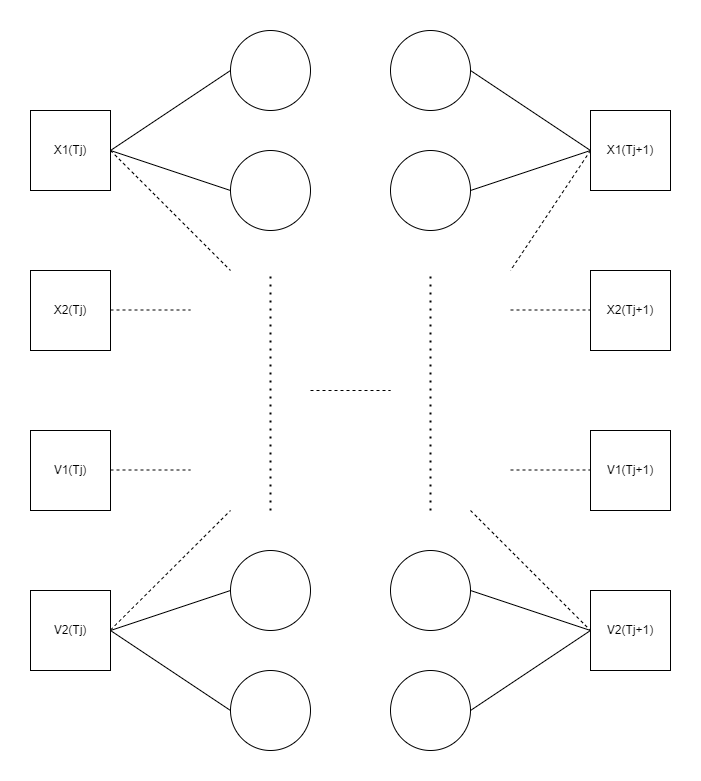
\includegraphics[scale=0.3]{../NN_graph.png}
    \caption[]{Neural Network structure}
    \label{fig:neural_network}
\end{figure}

\section{Discussion}
The performance of the feed forward neural network was evaluated based on its ability to replicate the physical behavior of sea-ice flow over a specified time frame, which has shown both significance and challenges. 

The references solutions were obtained by randomly generating the initial states and the flow function.
The initial states are generated by sampling from a Gaussian distribution with mean of 0 and variance of 1. The parameter $\alpha$ and $\beta$ are sampled from a uniform distribution between 0 and 1. The loss is evaluated using root mean square error (RMSE) of the displacement and the momentum. The time step chosen is $10^{-5}$, which is expected to be more accurate than the time step used in the training process.

The mean RMSE of the 16 test cases is 0.019571484194525812, which indicates a good performance of the model. In addition, the animinations and the loss graphs retrieved (Appendix GitHub link) also support the conclusion.

\section{Conclusion}
In conclusion, the feed forward neural network is capable to model the sea-ice flow with good accuracy, and robust enough to predict the movement of ice with different ocean velocity field. In addition, the use of weighted loss function has proven to be effective in reducing the error accumulation.

\newpage
\section{Appendix}
Code: 
\href{https://github.com/Kecheng-Zhang/Sea-ice-flow-simplified}{https://github.com/Kecheng-Zhang/Sea-ice-flow-simplified}

\end{document}